\chapter{Introduction}
\label{introchap}

In the early 1990s it was suggested that linguistics might be the first academic discipline to preside over its own demise. As much as 90\% of the world’s 7,000 languages are predicted to become extinct by the end of the 21st century \citep{krauss_worlds_1992,krauss_keynote--mass_2007,campbell_new_2013}. Therefore, it is critical that languages  be documented and described before they disappear. % without sufficient accessible data.Since the disquieting warning about language endangerment, 
Linguistic structures and language development cannot be studied without accessible data. Linguists have responded by putting greater emphasis on the documentation and description of endangered languages. In the past thirty years, documentary and descriptive fieldwork has achieved impressive results. Our knowledge of the world's language is steadily broadening beyond a handful economically or politically powerful languages. However, this work 
%including the process of annotating texts and analyzing morphological paradigms, 
must be increased and improved if it is to counteract the crisis of language endangerment. 
If the production of accessible data is to match the pace of language extinction, computational methods must be effectively integrated into the workflow of language documentation and description. 

Natural language processing (NLP) has not responded as quickly to the language endangerement crisis. Since the 1990s, machine learning systems, capable of learning complex patterns in data, have gained tremendous success in NLP. 
%Typically, state-of-the-art systems, specifically neural networks, require hundreds of thousands, or even millions, of data instances (words, sounds, sentences, etc.) to achieve state-of-the-art results. Few languages have more than a couple of thousand tokens,
%, let alone much available data, 
However, NLP research has been limited to handful of major languages such as Chinese, Arabic, English and other European languages. These languages are well documented and described. None 
%demonstrate complicated morphology polysynthetic type, none are under-documented, none 
are endangered.%\mans{The big data requirement is pretty specific to neural models.} 

Fortunately, this is changing. In recent years, NLP research with limited data has burgeoned. This is evidenced, for instance, by the 2015-2019 DARPA-funded LORELEI project, motivated in part by the 2014 Haiti earthquake where disaster aid was hampered by language. Haitian Creole is a language rarely encountered in NLP. When medicine and clean water were available, foreign aid workers struggled to process information that told them where supplies were most urgent. 

Despite this growth, very few NLP systems have been integrated into the process of documenting and describing endangered languages. This may be due to the specific challenges presented by the dynamic, evolving nature of ongoing linguistic analysis and the inconsistencies that arise during the manual annotation. These challenges illustrate why documentary and descriptive linguists must adjust their methods
%their methods to the specifications of machine learning specifications 
in order to effectively integrate the benefits of machine learning.

\section{Overview of Proposed Research}

In production of new language data, illustrated in Figure \ref{fig:flowchart}, a team of linguists and native speakers (a) collaborate to document language data that benefits the community of speakers, linguistic sciences, and NLP development. However, a bottleneck of time-consuming annotation (b) makes keeps data largely inaccessible. The proposed research examines ways that linguists can address this by integrating machine learning (c). Machine learning increases %provide automated assistance to document and describe endangered languages with 
speed and accuracy but linguists must be able to make effective use of it. The proposed dissertation research 
%will focus on effective integration of machine learning into language documentation and description. It 
will ask how linguists should adjust their work to achieve optimal results from machine learning assistance. It will look specifically at interlinearization and inflectional paradigm induction.
%The proposed research focuses on effective integration for morphological annotation and analysis.

\begin{figure}[h!]
\centering
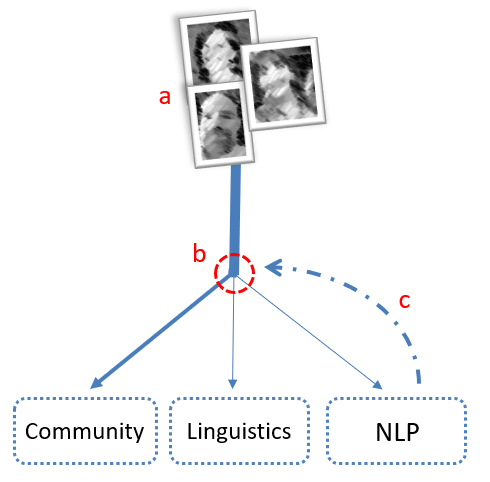
\includegraphics[width=6cm]{figs/Flowchart.PNG}
\caption[Language Data Production]{Language Data Production}
\label{fig:flowchart}
\end{figure}


Once language data has been analyzed and annotated it becomes usable for further scientific discovery in linguistics and NLP. After documented data is transcribed, it is annotated with basic linguistic analysis in a multi-step process called interlinearization. Narrowly defined, interlinearization comprises three tasks: 1) segmenting words into morphemes, 2) glossing each morpheme with its narrow lexical or grammatical translation, and 3) freely translating whole sentences into a language of wider communication to show how the morphemes combine to create meaning. The result is illustrated in example (\ref{ex:IGTex}) with a transliterated Russian sentence. Interlinearization lays the foundation for other analysis and annotation, such as identifying morphological inflectional patterns.  
%Although textual data contains many repeated linguistic structures, it is only by 
%Interlinearizing all data uncovers rare and unique linguistic phenomena among the very common and frequently repeated structures. 

\begin{singlespace}
\pex<IGTex>   
\label{ex:IGTex}
\textbf{Text:} \hspace{14 mm} Vecherom \hspace{4.75 mm} ya \hspace{13 mm} pobejala \hspace{21 mm} v \hspace{2 mm} magazin \\
\textbf{Segmented:} \hspace{2 mm} vecher-om \hspace{4 mm} ya \hspace{13 mm} pobeja-la \hspace{20 mm} v \hspace{2 mm} magazin \\
\textbf{Glossed:} \hspace{8.5 mm} evening-\textsc{ins} \hspace{1 mm} 1.\textsc{sg.nom} \hspace{1 mm} run-\textsc{pfv.pst.sg.fem} \hspace{1 mm} in \hspace{1 mm} store.\textsc{acc} \\
\textbf{Translation:} \hspace{1 mm} `In the evening I ran to the store.' \\
\xe
\end{singlespace}


The proposed dissertation is motivated by a “yawning gap” \citep{seifart_language_2018} between the amount of documented data deposited in language archives and the portion of the data that is usable for research. This gap is caused by what has been described as an annotation bottleneck, illustrated in Figure \ref{fig:bottleneck}. The bottleneck is created by currently accepted but tedious and time-consuming methods that are done primarily by hand from start to finish \citep{simons_worlds_2013,holton_developing_2017}. 
%The process is labor- and time-intensive. Manual annotation is subject to human error, with many mistakes and inconsistencies due not to the difficulty of the task, but to its repetitive and monotonous nature.
Budget constraints often mean that large portions of the data produced by field projects are left unannotated. They remain untapped resources. These resources could inform the development of linguistics science and NLP. They could also build human language technology that would benefit the communities that speak them. 

The proposed research asks: \emph{How should the integration of machine learning  influence accepted workflows of language documentation and description?} It will use machine learning and corpora from six endangered or under-documented languages to  
%address the annotation bottleneck by examining 
examine how current methods affect machine learning performance and the potential to incorporate more automated assistance. This will be done with three studies:

\begin{enumerate}
\item{} \textbf{Automating Segmentation and Glossing:} How do choices made during interlinearization (i.e. surface versus canonical segmentation, in/consistent morpheme boundaries, lack/presence of part of speech tags) affect machine learning results on morpheme segmentation and glossing? How do these choices affect the performance of different machine learning models?

\item A SECOND QUESTION

%\item{} \textbf{Balance of Interlinearization Tasks:} When faced with limited time, how does integration of machine learning dictate the priorities of completing different interlinear lines? 
%segmentation and glossing over free translation? 
%    \begin{itemize}
%        \item{} What ratio of completed lines achieves optimal machine learning performance on all interlinear lines?
%        \item{} To what extent does completion of other interlinear lines affect the results on any one line? I.e.  Does leveraging glosses improve machine translation? Can information extracted from other lines of interlinear glossed texts improve segmentation and glossing?  
%    \end{itemize}

\item{} \textbf{Morphological Description:} To what extent can manually interlinearized texts be utilized for computational induction of morphological inflection patterns? 
\end{enumerate}


\begin{figure}[h!]
    \centering
    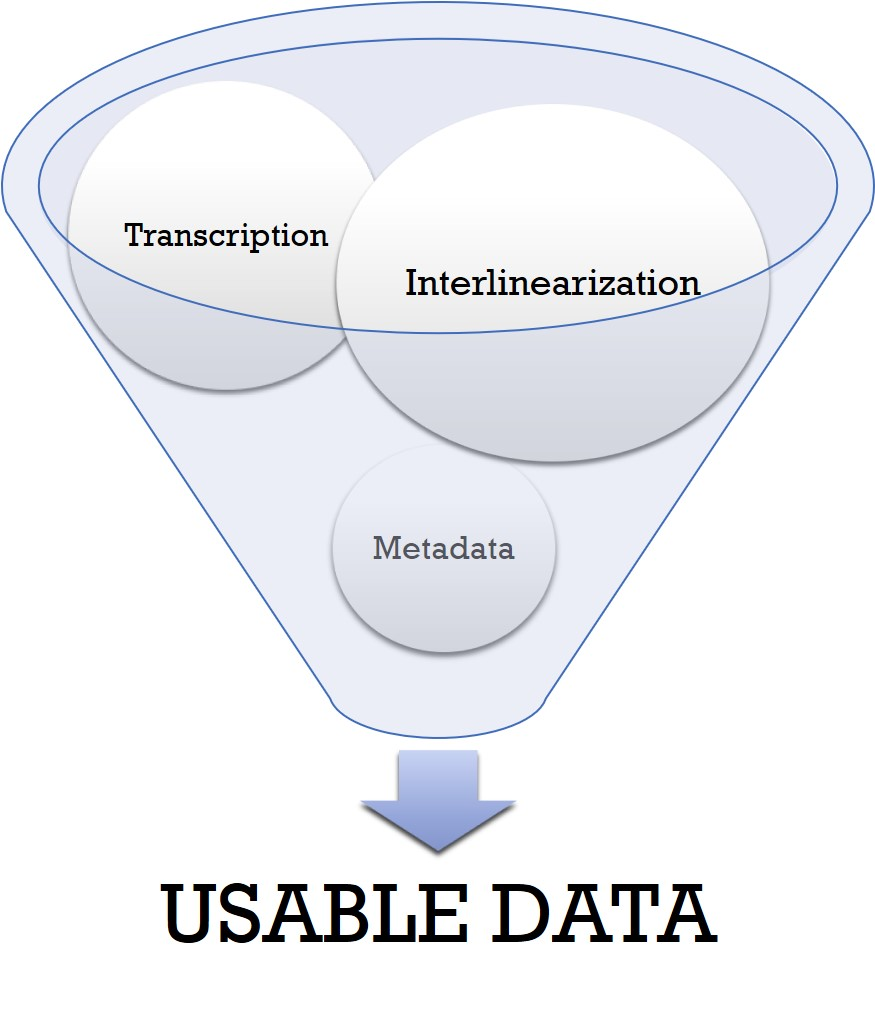
\includegraphics[width=6cm]{figs/AnnotationFunnel.jpg}
    \caption[Annotation Bottleneck]{Annotation bottleneck in language documentation and description.}
    \label{fig:bottleneck}
\end{figure}

\section{Expected Results and Implications}

The proposed dissertation research will study effective integration of computational methods that could open the annotation bottleneck. 
%caused by current time-consuming manual methods to produce morpheme segmentation, glossing, free translation, and first-pass hypotheses of morphological inflectional paradigms. 
Its contribution will be four-fold. 

First, it will demonstrate how machine learning can be applied to tasks into the documentary and descriptive pipeline in several languages. This will test the potential to produce new annotated data more quickly and accurately than current methods. Other research has demonstrate this with models built for one or two languages. This research will demonstrate the potential for several languages with the same models. The result will be a machine learning pipeline for interlinearization and inflectional paradigm induction.

Second, the proposed dissertation will demonstrate the potential for machine learning to assist linguists in deeper linguistic analysis and description. A main theme of the proposed research is that machine learning systems can take advantage of the typical output from documentary and descriptive field work but this requires cooperation and flexibility. It will unite the efforts of linguistics and NLP by training machine learning on linguistic field data. Rather than curated published data  NLP systems are normally trained on, it will leverage interlinearized glossed texts produced by documentary and descriptive projects. Since this research will be performed on “real live” field data---sometimes the only annotated data available for a language---it may uncover unforeseen challenges for NLP in low-resource settings.
%Specifically, it will use neural networks to learn inflectional patterns in six languages.
%\mans{``neural machine learning'' is perhaps a little too loose: neural networks might be better.}
This is a step towards integrating machine learning assistance when building holistic hypotheses about a language's structure.

Third, it will establish not only that new computational methods can be successfully integrated into language documentation and description, but show how this will impact linguistics field methods. It will do this by analyzing the characteristics of the input data. Much of the discussions will focus on how these characteristics affect the machine learning's output.

Fourth, the proposed research will increase annotated data in six endangered and low-resource languages. These languages represent a range of linguistic structures and language families. They are spoken by communities across five continents. Interlinear texts in these languages are currently limited to 5-100K words. The amount of descriptive linguistic publications for all is quite low. Increasing annotated data would allow more thorough testing of linguistic theories and computational models.
%, which contribute to our understanding of human language and the performance of machine learning algorithms in low-resource settings. 

\section{Organization of Prospectus}

This Prospectus describes the author's planned dissertation research. Chapter \ref{chap:litreview} reviews issues in previous research that are related to the proposed research. Chapter \ref{chap:datamodels} describes the data and computational models that will be used. Chapter \ref{chap:body} outlines the experiments that will be conducted and presents results from pilot studies. The Prospectus concludes with a timeline (Chapter \ref{chap:timeline}). % and a summary (Chapter \ref{chap:conclusion}) of the potential impact of this work.

